\documentclass[11pt,a4paper]{article}
\usepackage{lmodern}
\usepackage[utf8]{inputenc}
\usepackage[T1]{fontenc}
\usepackage{amsmath}
\usepackage{amssymb}
\usepackage{amsthm}
\usepackage{esint}
\usepackage{graphicx}
\usepackage[francais,english]{babel}

\setlength{\oddsidemargin}{0mm}
\setlength{\evensidemargin}{0mm}
\setlength{\topmargin}{-15mm}
\setlength{\textheight}{25cm}
\setlength{\textwidth}{16cm}

\newcommand{\N}{\mathbb N}       
 \renewcommand{\S}{\mathbb S}     
\newcommand{\R}{\mathbb R} 
\newcommand{\C}{\mathbb C} 
\newcommand{\K}{\mathbb K}
\newcommand{\ds}{\displaystyle}

%\pagestyle{plain}
%#############################################################################################
\begin{document}
\selectlanguage{french}

\noindent 
Sorbonne Universit\'e - Université Paris Cité     \hfill   Ann\'ee 2021-2022 \\
Pr\'eparation \`a  l'agr\'egation        \hfill     Vendredi 15 avril 2022 \\ % \emph{Dur\'ee : 3h}
 %\hfill \emph{Calculatrices et t\'el\'ephones interdits} \\
\noindent {\rule{\textwidth}{.2mm}}\\[-5mm]
\begin{center}
{\large \textsc{Corrigé examen option B} }\\[-5mm]
\end{center}
\noindent {\rule{\textwidth}{.2mm}}\\[1cm]



%%%%%%%%%%%%%%%%%%%%%%%%%%%%%%%%%%
{\bf Exercice 1 : un portrait de phase ($\sim$11 pts)} \vspace{0.1cm}\\
On considère l'\'equation de Van der Pol : 
\begin{equation}\label{EDO}
  y'' + (y^2-1) y' + y = 0 ,
\end{equation}
compl\'et\'ee par les conditions initiales $(y(0), y'(0))=Y_0 \in \R^2$.

\begin{enumerate}
\item R\'e\'ecrire ce probl\`eme de Cauchy sous la forme d'un syst\`eme d'ordre 1:
  $Y' = F(t,Y(t))$, $Y(0) = \tilde{Y}_0$.
\item Prouver qu'il existe une unique solution maximale $Y(t)$ \`a ce syst\`eme.
\item Donner les points d'\'equilibre de ce syst\`eme. \'Etudier leur stabilit\'e.
\item Calculer les isoclines et les tracer sur le portrait de phase.
\item Tracer le portrait de phase dans la r\'egion la plus en bas \`a droite
  (d\'elimit\'ee par une isocline).
\item Montrer que si $(y_1(0),y_2(0))$ est dans la r\'egion
  \begin{align*}
    \left\{ (y_1,y_2) \; | \; y_2 < \min \left(0 , \frac{y_1}{1-y_1^2} \right)
    \; | \; | y_1 | < 1 \right\} \cup
    \Big\{ (1,y_2) \; | \; y_2 < 0 \Big\} \cup
    \left\{ (y_1,y_2) \; | \; \frac{y_1}{1-y_1^2} < y_2 < 0 \; | \; y_1 > 1 \right\} ,
  \end{align*}
  alors la solution atteint une isocline en temps fini.
  Tracer le portrait de phase dans cette r\'egion.

\item Montrer que si $(y_1(0),y_2(0))$ est dans la r\'egion la plus en bas \`a gauche
  du portrait de phase (d\'elimit\'ee par deux isoclines),
  alors la solution atteint une isocline en temps fini.
  Tracer le portrait de phase dans cette r\'egion.
\item Montrer que $F$ est impaire. Compl\'eter le portrait de phase
  en utilisant la sym\'etrie par rapport \`a $(0,0)$.
\item En utilisant le portrait de phase, justifier que, pour toute condition initiale,
  la solution maximale est d\'efinie sur $\R_+$.
\end{enumerate}

%%%%%%%%%%%%%%%%%%%%%%%%%%%%%%%%%% 
{\bf Exercice 2 : m\'ethode de Newton ($\sim$3 pts)} \vspace{0.1cm}\\
On considère la fonction $f(x) = x^2-1$.

\begin{enumerate}
\item Écrire la méthode de Newton pour la recherche de zéros de cette fonction, en partant de $x_0$ donné.

\item On prend $x_0=1+\varepsilon$. Donner un équivalent de $(x_1-1)$ en fonction de $\varepsilon$ lorsque $\varepsilon \to 0$ si on applique l'algorithme de Newton à $x_0$ pour calculer $x_1$. En déduire un équivalent de $(x_n-1)$.
\end{enumerate}

\newpage

%%%%%%%%%%%%%%%%%%%%%%%%%%%%%%%%%%
{\bf Exercice 3 : m\'ethode du gradient ($\sim$8 pts)} \vspace{0.1cm}\\

Pour $A\in{\cal M}_n({\mathbb R})$, on note $\displaystyle\|A\|_2=
\max_{x\in{\mathbb R}^n,x\neq 0}\frac{\|Ax\|_2}{\|x\|_2}$ la norme matricielle induite 
par la norme vectorielle $\|.\|_2$. 
 
\begin{enumerate}
\item Soit une matrice orthogonale $U\in{\cal M}_n({\mathbb R})$ ($U^TU=I_n$). 
\begin{enumerate}
 \item 
Montrer que pour tout  $x\in{\mathbb R}^n$, on a
$\|Ux\|_2=\|x\|_2$.
\item Montrer que si $V$ est un matrice orthogonale, on a pour tout $A\in {\cal M}_n({\mathbb R})$, on a $\|UAV\|_2=\|A\|_2$.
\item 
En d\'eduire que si la matrice $A$ est sym\'etrique, on a $\|A\|_2=\varrho(A)$, le rayon spectral de $A$. 
\end{enumerate}
\item 
On pose $u(x)=
\frac{1}{2} \langle A x,x \rangle - \langle x,b \rangle$,
o\`u $A\in{\cal M}_n({\mathbb R})$ est sym\'etrique d\'efinie positive et $b\in{\mathbb R}^n$. 

\begin{enumerate}
\item Montrer que le probl\`eme $\min_{x\in{\mathbb R}^n} u(x)$ a une solution et une seule qu'on note  $x^\ast$. 
\item On consid\`ere la m\'ethode du gradient pour calculer $x^\ast$ ($\alpha\in{\mathbb R}$) : $x_0\in{\mathbb R}^n$ et 
\begin{equation*} 
x_{k+1}=x_k -\alpha\nabla u (x_k)
\end{equation*}
\'Ecrire la m\'ethode sous la forme $x_{k+1}=Bx_k +c$, o\`u $B$ est une matrice et $c$ un vecteur. En d\'eduire que  $x_{k}-x^\ast=B^k(x_0 -x^\ast)$. Puis que la m\'ethode converge si et seulement si $\alpha \in I=]0, 2/\varrho(A)[$.
 \item Montrer que pour tous vecteurs $x$ et $y$ de ${\mathbb R}^n$, on a 
\[u(y) = u(x) + \frac{1}{2} 
\langle A (y-x),y-x \rangle +  \langle \nabla u(x), y-x \rangle.\] 
En d\'eduire que si $x_k\neq x^\ast$, on a pour tout $\alpha \in I$,   
\[u(x_{k+1}) < u(x_k).\]

\end{enumerate}
\end{enumerate}

\newpage

%%%%%%%%%%%%%%%%%%%%%%%%%%%%%%%%%
{\bf Correction de l'exercice 1:} \vspace{0.1cm}\\

\begin{enumerate}
\item En posant $Y(t) = (y(t) , y'(t))$, on peut r\'e\'ecrire le syst\`eme comme
  $Y'(t) = F(Y(t))$ avec $F(Y) = (y_2 , -y_1 - (y_1^2 - 1) y_2)$ o\`u
  on a pos\'e $Y = (y_1 , y_2) \in \R^2$.
  La donn\'ee de Cauchy devient $Y(0) = Y_0$.

\item La fonction $F$ ne d\'epend pas de $t$ et est d\'erivable
  (donc localement Lipschitzienne en $Y$, uniform\'ement en $t$). Elle est aussi continue.
  Le th\'eor\`eme de Cauchy-Lipschitz local nous donne donc l'existence d'une unique solution
  maximale \`a ce probl\`eme de Cauchy.

\item Les points d'\'equilibre $(x_1,x_2)$ du syst\`eme sont les points v\'erifient
  le syst\`eme
  \begin{align*}
    y_2 = 0 ,
    \\
    - y_1 - (y_1^2 - 1) y_2 = 0 .
  \end{align*}
  Le seul point d'\'equilibre du syst\`eme est donc $(0,0)$.

  Pour \'etudier sa stabilit\'e, on calcule la matrice jacobienne de $F$:
  \begin{align*}
    J_F(Y) =
    \begin{pmatrix}
      0 & 1
      \\
      -1-2y_1y_2 & 1-y_1^2
    \end{pmatrix}
  \end{align*}
  En $(0,0)$, on a
  \begin{align*}
    A = J_F(0,0) =
    \begin{pmatrix}
      0 & 1
      \\
      -1 & 1
    \end{pmatrix} .
  \end{align*}
  Le polyn\^ome caract\'eristique de cette matrice est
  $P_A(\lambda) = \lambda^2 - \lambda + 1$.
  Les valeurs propres de $A$ sont donc $\dfrac{1 \pm i \sqrt{3}}{2}$.
  Le point d'\'equilibre $(0,0)$ est donc instable.

\item Les isoclines sont donn\'ees par $y_2 = 0$ ($y_1' = 0$)
  et $y_2 = \dfrac{y_1}{1-y_1^2}$ ($y_2' = 0$).

\item Voir portrait de phase. Cette r\'egion est appel\'ee $\mathcal{I}$ dans la suite.

\item Cette r\'egion est appel\'ee $\mathcal{II}$ dans la suite.
  Si $(y_1(0),y_2(0))$ est dans $\mathcal{II}$, alors, comme $y_1'(t) < 0$ et $y_2'(t) < 0$ :
  soit il existe un temps $t_1 > 0$ tel que $(y_1(t_1) , y_2(t_1))$ atteigne
  l'isocline $y_2' = 0$, soit la solution $(y_1(t),y_2(t))$ reste dans la zone $\mathcal{II}$
  et $y_2(t) \to - \infty$.

  
  Dans cette r\'egion, $y_1(t)$ reste born\'e car d\'ecroissant et minor\'e.
  Et $y_2'(t) = -y_1 - (y_1^2 - 1) y_2(t) \geq A + B y_2(t)$, avec $A,B \in \R$.
  Ainsi $y_2(t)$ se comporte au pire comme une exponentielle et ne peut donc pas exploser en temps
  fini.
  De plus, $y_2(t)$ est d\'ecroissante et $y_1'(t) = y_2(t) \leq y_2(0)$;
  ce qui implique $y_1(t) \leq y_2(0) t$.
  Donc $(y_1(t),y_2(t))$ atteint en temps fini l'isocline d\'efinissant la fronti\`ere gauche de
  $\mathcal{II}$.


\item On note cette r\'egion $\mathcal{III}$ (voir le portrait de phase).
  On a $y_1(t)$ d\'ecroissante et $y_2(t)$ croissante.
  Ainsi, soit on atteint l'isocline d'\'equation $y_2 = 0$, soit $y_1(t) \to - \infty$.
  Si, pour $t_1 > 0$, $y_1(t_1) < -1$, alors $y_2'(t) \geq - y_1(t) \geq 1$
  et $y_2(t) \geq y_2(0) + t$.
  Si ce n'est pas le cas, c'est qu'on atteint l'isocline d'\'equation $y_2 = 0$
  et ceci ne peut se faire qu'en temps fini puisque le point d'\'equilibre $(0,0)$ est r\'epulsif
  (toutes les VP de la jacobienne sont de partie r\'eelle > 0).

  Toujours dans le cas $y_1(t_1) < -1$, $y_1'(t) = y_2(t) \geq y_2(0)$.
  Ainsi $y_1$ n'explose pas en temps fini tandis que $y_2(t) \geq y_2(0) + t$
  implique que $(y_1(t),y_2(t))$ atteint l'isocline d'\'equation $y_2=0$ en temps fini.
  
\item Tout simplement,
  $F(-Y) = (- y_2 , y_1 - ((-y_1)^2 -1)(-y_2)) = - F(Y)$.
  Voir le portrait de phase pour le trac\'e.

\item On montre que pour toute donn\'ee initiale, la solution maximale
  est born\'ee sur tout intervalle $J$ de $\R_+$
  ce qui implique qu'elle est d\'efinie sur $\R_+$ entier.

  Pour montrer qu'elle est born\'ee, utilisons le portrait de phase.
  Il est extr\^emement important de noter ici que les orbites du portrait de phase
  ne peuvent pas se croiser (\`a part au point d'\'equilibre) sinon on obtient localement
  deux solutions distinctes, ce qui n'est pas possible
  puisque l'on est toujours sous les hypoth\`eses du th\'eor\`eme de Cauchy-Lipschitz local.

  
  Toute solution de la zone $\mathcal{I}$ passe dans la zone $\mathcal{II}$,
  puis dans la zone $\mathcal{III}$, puis dans les zones $\mathcal{V}$ et $\mathcal{VI}$
  avant de revenir dans la zone $\mathcal{II}$.
  Comme les orbites ne peuvent pas se croiser, la solution doit rester en dessous
  de toute solution provenant de la zone $\mathcal{IV}$, et ce dans les zones $\mathcal{V}$
  et $\mathcal{VI}$.
  De m\^eme, quand elle revient dans les zones $\mathcal{II}$ et $\mathcal{III}$,
  elle doit rester au-dessus de toute orbite provenant directement de la zone $\mathcal{I}$.
  La solution est donc born\'ee sur tout intervalle de $\R_+$.

  Le m\^eme raisonnement s'applique si on prend la condition initiale dans une autre zone.
  La solution maximale est donc d\'efinie sur $\R_+$.

\end{enumerate}

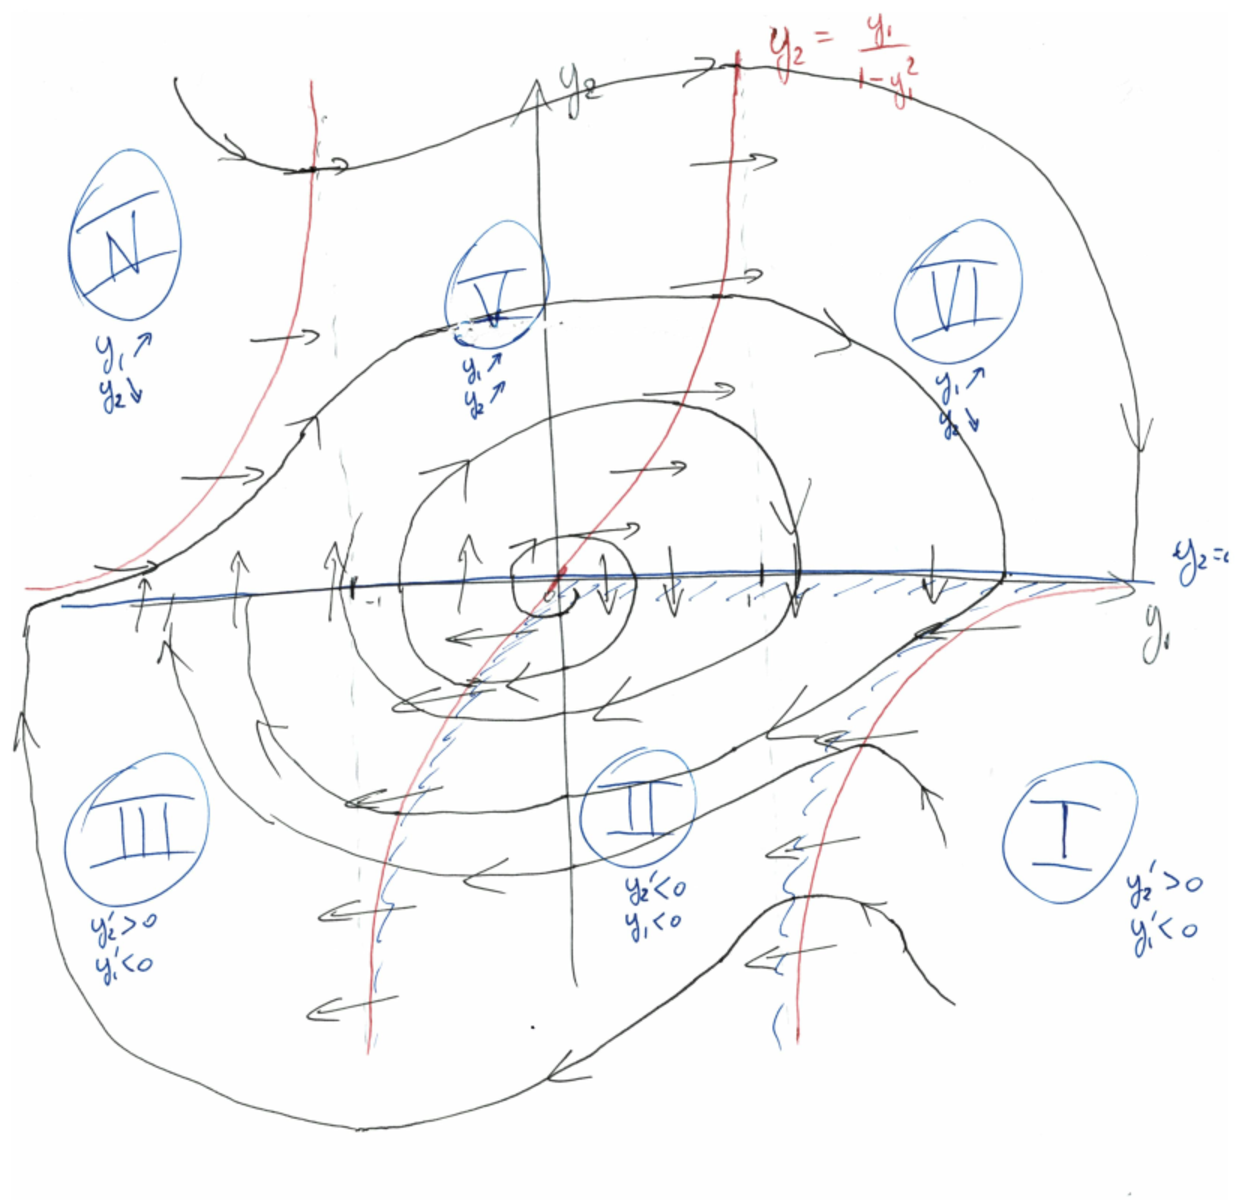
\includegraphics[width=0.99\textwidth]{portrait_phases.pdf}

\newpage

%%%%%%%%%%%%%%%%%%%%%%%%%%%%%%%%%
{\bf Correction de l'exercice 2:} \vspace{0.1cm}\\
\begin{enumerate}
\item La méthode de Newton pour la recherche d'un zéro d'une fonction dérivable $f$ s'écrit :
$$
\left\{
\begin{array}{l}
x_0 \mbox{ donné,}\\
x_{n+1} = x_n -\dfrac{f(x_n)}{f'{x_n)}}.
\end{array}
\right.
$$
Donc ici
$$
\left\{
\begin{array}{l}
x_0 \mbox{ donné,}\\
x_{n+1} = x_n -\dfrac{x_n^2-1}{2x_n} = \dfrac{x_n^2+1}{2x_n} = \dfrac{1}{2}\left(x_n + \dfrac{1}{x_n}\right).
\end{array}
\right.
$$
\item On écrit le développement limité suivant (aller jusqu'à l'ordre 2 est nécessaire!) :
$$
\dfrac{1}{1+\varepsilon} = 1-\varepsilon+\varepsilon^2 + o(\varepsilon^2)
$$
d'où, en utilisant l'expression de la question a) :
$$
x_1 = \dfrac{1}{2}\left(1+\varepsilon + \dfrac{1}{1+\varepsilon}\right) = \dfrac{1}{2}\left(1+\varepsilon + (1-\varepsilon+\varepsilon^2 + o(\varepsilon^2))\right) = 1 + \dfrac{\varepsilon^2}{2} + o(\varepsilon^2)
$$
donc $x_1-1 \approx \dfrac{\varepsilon^2}{2}$ lorsque $\varepsilon \to 0$.
\\
On peut itérer ce raisonnement : 
on voit que si on pose $x_1 = 1+\eta$, avec $\eta = \dfrac{\varepsilon^2}{2}+o(\varepsilon^2)$, alors 
$$x_2 = 1 + \dfrac{\eta^2}{2} + o(\eta^2) = 1 + \dfrac{\varepsilon^4}{8} + o(\varepsilon^4) \;\; \mbox{ et }\;\; x_2-1\approx\dfrac{\varepsilon^4}{8}= 2\left(\dfrac{\varepsilon}{2}\right)^4.$$
Au vu de ce calcul, faisons l'hypothèse que
$$
x_n = 1 + 2\left(\dfrac{\varepsilon}{2}\right)^{2^n} + o(\varepsilon^{2^n})
$$
Nous allons montrer l'estimation ci-dessus par récurrence : 

$\bullet$ Initialisation : on a bien $x_0 =1+ 2\left(\dfrac{\varepsilon}{2}\right)^{1}$. 

$\bullet$ Induction :
supposons $x_n = 1 + 2\left(\dfrac{\varepsilon}{2}\right)^{2^n}+ o(\varepsilon^{2^n})$.\\
Montrons que cela entraîne $x_{n+1} =1 + 2\left(\dfrac{\varepsilon}{2}\right)^{2^{n+1}}+ o(\varepsilon^{2^{n+1}})$ :\\
On pose $\eta = x_n-1 = 2\left(\dfrac{\varepsilon}{2}\right)^{2^n}+ o(\varepsilon^{2^n})$. On a alors
$$
\begin{array}{rl}
x_{n+1} &= \dfrac{1}{2}\left(x_n + \dfrac{1}{x_n}\right) = \dfrac{1}{2}\left(1+\eta + \dfrac{1}{1+\eta}\right)\\
&= \dfrac{1}{2}\left(1+\eta+(1-\eta+\eta^2+o(\eta^2))\right) = 1+\dfrac{\eta^2}{2}+o(\eta^2))\\
&= 1+2\left(\dfrac{\varepsilon}{2}\right)^{2^{n+1}}+ o(\varepsilon^{2^{n+1}}).
\end{array}
$$
La récurrence est bien vérifiée et on en déduit l'équivalent :
$$
x_n -1 \approx 2\left(\dfrac{\varepsilon}{2}\right)^{2^n}\quad\mbox{lorsque } \varepsilon\to 0.
$$
On a ainsi démontré "manuellement", pour cette fonction $f$ particulière, la convergence quadratique de la méthode de Newton.
\end{enumerate}

%%%%%%%%%%%%%%%%%%%%%%%%%%%%%%%%%
{\bf Correction de l'exercice 3:} \vspace{0.1cm}\\

\begin{enumerate}
\item  
\begin{enumerate}
 \item On note que $\|Ux\|_2^2=\langle Ux,Ux\rangle=\langle U^Tx,x\rangle=\|x\|_2$.
\item Pour le calcul de $\|UA\|_2$, on \'ecrit 
$\|UAx\|_2^2=\langle UAx,UAx\rangle=\langle U^TUA,Ax\rangle=\|Ax\|_2$. Pour le calcul de $\|AV\|_2$, on effectue un changement de variable bijectif
$\|AVx\|_2=\|Ay\|_2$ avec $y=Vx$. On a donc $\|UAV\|_2=\|AV\|_2=\|A\|_2$.
\item Si $A$ est sym\'etrique, elle est diagonalisable dans une base orthonorm\'ee de vecteurs propres. Ce qui s'écrit $A=PDP^{-1}$
avec $P$ orthogonale et $D$ la matrice diagonale 
compos\'ee des valeurs propres de $A$. On a donc
$\|A\|_2=\|D\|_2$. Or $\|D\|_2=\max_{i}|D_{i,i}|$ (exercice!). D'o\`u le r\'esultat. 
\end{enumerate}
\item 
On pose $u(x)=
\frac{1}{2} \langle A x,x \rangle - \langle x,b \rangle$,
o\`u $A\in{\cal M}_n({\mathbb R})$ est sym\'etrique d\'efinie positive et $b\in{\mathbb R}^n$. 

\begin{enumerate}
\item L'existence d'un minimum est assur\'ee par le fait que $u$ soit coercive (``tend vers l'infini \`a l'infini'')
\[|u(x)|\leq \frac12 \lambda_{min}\|x\|_2^2-\|b\|_2\,\|x\| \underset{\|x\|\to +\infty}{\to}+\infty.\]
L'unici\'e est assur\'ee par la stricte convexit\'e de la hessienne de $u$, qui est \'egale \`a la matrice sdp $A$. 
\item On a $\nabla u(x)=Ax-b$ et $\nabla u(x^\ast)=0$. La m\'ethode du gradient s'\'ecrit aussi $x_{k+1}=Bx_k +c$ avec $BI-\alpha A$ et $c=\alpha b$.  Comme $x^\ast=Bx^\ast +c$, on en d\'eduit que $x_{k+1}-x^\ast=B(x_k -x^\ast)$ et donc $x_{k}-x^\ast=B^k(x_0 -x^\ast)$. La convergence a lieu donc si et seulement si la suite $(B^k)_k$ tend vers $0$. Ce qui est le cas si et seulement si \fbox{je d\'etaillerai plus plus tard} $\varrho(B)<1$. Or le spectre de $B$ est form\'e des $1-\alpha\lambda$ avec $\lambda$ dans le spectre de $A$. Le condition 
\[|1-\alpha\lambda|< 1,\quad \forall \lambda \in\mbox{Sp}(A)\]
conduit au r\'esultat : la m\'ethode converge si et seulement si $\alpha \in I=]0, 2/\varrho(A)[$.
 \item Montrer que pour tous vecteurs $x$ et $y$ de ${\mathbb R}^n$, on a 
\[u(y) = u(x) + \frac{1}{2} 
\langle A (y-x),y-x \rangle +  \langle \nabla u(x), y-x \rangle.\] 
On prend $y=x-\alpha \nabla u(x)$ dans l'in\'egalit\'e :
\[u(x-\alpha \nabla u(x)) = u(x) + \frac{\alpha^2}{2} 
\langle A \nabla u(x),\nabla u(x) \rangle -\alpha \langle \nabla u(x), \nabla u(x) \rangle.\] 
On en d\'eduit  que 
\[u(x-\alpha \nabla u(x)) \leq u(x) + \alpha(\frac{\alpha}{2}\|A\|_2-1) \|\nabla u(x)\|_2^2.\]

En d\'eduire que si $x_k\neq x^\ast$, on a pour tout $\alpha \in I$,   
\[u(x_{k+1}) < u(x_k).\]

\end{enumerate} 
 
 
\end{enumerate}


\end{document}
